% -*- coding: UTF-8 -*-
% hurlex-chapt4.tex
% hurlex 开发文档 第4章内容

\section {字符模式下的显卡驱动}

\par 本章将开始描述对屏幕输出的控制。在第二章我们简单谈过地址空间的事情,并提到4G的地址空间并非全部指向主存储器,而是有部分\allowbreak
的地址分给了其他外设。特别地,在地址空间的最低1MB处,有很多地址是属于外部设备的,下图描绘了该处地址映射的分布情况:

\begin{figure}[ht]
      \centering
      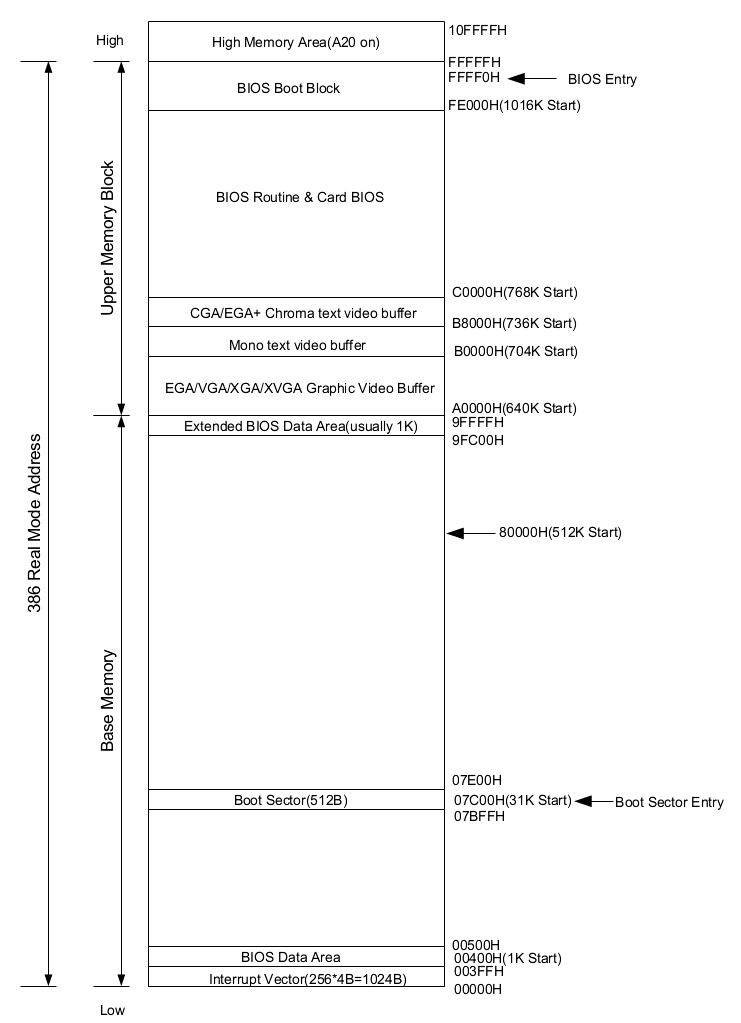
\includegraphics[scale=0.65]{picture/chapt4/BIOS-mem.png}
      \caption{低端地址空间的映射关系}
\end{figure}

\par 在PC上要显示文字,通常需要显示器和显卡这两个硬件设备。一般说来显卡负责提供显示\allowbreak
内容,并控制具体的显示模块和状态;显示器的职责是负责将显卡呈递的内容可视化的显示出来。既然显卡需要控制显示的数据,自然就需要\allowbreak
存储这些待显示的内容,所以显卡就有自己的存储区域。这个存储区域叫做显示存储器(Video RAM,VRAM),简称显存。当然,访问显存\allowbreak
就需要地址。上面提到的这个区域映射的就是工作在文本模式的显存。同时显卡还有另外一个工作模式叫做图形模式,这个模式是目前\allowbreak
最常用的模式。

\par 我们知道,对于一个字符的编码通常有输入码、内码和字模码三种。其中字模码定义了一个字符在屏幕上显示的点阵坐标。一般说来,显卡\allowbreak
内置一套关于基本英文字符的显示是很容易做到的,而内置汉字的显示就较为麻烦。\footnote{曾经有类似于"汉卡"之类的硬件出现,\allowbreak
后来随着计算机处理速度的发展,这些工作一般由软件来负责了。}在这篇文档中我们只使用显卡的文本模式,不会涉及到图形模式的内容。\allowbreak
因为一旦使用了图形模式的内容,我们就需要自行定义字符的字模码了,这很繁琐而且对我们理解操作系统原理的意义不是很大。\allowbreak
所以我们只使用显卡的文本模式进行屏幕显示控制。所有在PC上工作的显卡,在加电初始化之后都会自动初始化到80*25的文本模式。\allowbreak
在这个模式下,屏幕被划分为25行,每行可以显示80个字符,所以一屏可以显示2000个字符。上图中的0xB8000~0xBFFFF这个地址段\allowbreak
便是映射到文本模式的显存的。当访问这些地址的时候,实际上读写的是显存区域,而显卡会周期性的读取这里的数据,并且把它们按\allowbreak
顺序的显示在屏幕上。

\par 那么,按照什么规则显示呢?这就要谈到内码了。内码定义了字符在内存中存储的形式,而英文编码就是大家所熟知的ASCII\allowbreak
(American Standard Code for Information Interchange,美国信息交换标准代码)码了。对应的关系很简单,从0xB8000这个地址开始,\allowbreak
每2个字节表示屏幕上显示的一个字符。从屏幕的第一行开始对应,一行接着一行的对应下去。而这两个字节的前一个是显示字符的ASCII码,\allowbreak
后一个是控制这个字符颜色和属性的控制信息,这个字节的8个bit位表示不同的含义。下图指出了每一位的含义:

\par 另外的一张图指出了文本模式下的颜色表:

\par 理解了显卡的文本模式的原理之后我们就要开始一些对屏幕控制的编码了。不过显卡除了显示内容的存储单元之外,还有部分的显示\allowbreak
单元需要了解。这些显示控制单元被编制在了独立的I/O空间里,需要用特殊的in/out指令去读写。这里需要寄存器多达300多个,\allowbreak
显然无法一一映射到I/O端口的地址空间。对此工程师们解决方案是,将一个端口作为内部寄存器的索引:0x3D4,再通过 0x3D5\allowbreak
端口来设置相应寄存器的值。

\par 首先是几个端口读写函数的实现。因为C语言并没有直接操作端口的方法,而且频繁的内联汇编麻烦又容易出错。所以好的做法就是定义\allowbreak
几个端口读写函数。代码如下:

\begin{lstlisting}[language = C, label = libs/common.c, caption = libs/common.c]
#include "common.h"

// 端口写一个字节
inline void outb(uint16_t port, uint8_t value)
{
	asm volatile ("outb %1, %0" : : "dN" (port), "a" (value));
}

// 端口读一个字节
inline uint8_t inb(uint16_t port)
{
	uint8_t ret;

	asm volatile("inb %1, %0" : "=a" (ret) : "dN" (port));

	return ret;
}

// 端口读一个字
inline uint16_t inw(uint16_t port)
{
	uint16_t ret;

	asm volatile ("inw %1, %0" : "=a" (ret) : "dN" (port));

	return ret;
}
\end{lstlisting}

\par 对应的头文件如下:
\begin{lstlisting}[language = C, label = include/common.h, caption = include/common.h]
#ifndef INCLUDE_COMMON_H_
#define INCLUDE_COMMON_H_

#include "types.h"

// 端口写一个字节
void outb(uint16_t port, uint8_t value);

// 端口读一个字节
uint8_t inb(uint16_t port);

// 端口读一个字
uint16_t inw(uint16_t port);

#endif // INCLUDE_COMMON_H_
\end{lstlisting}

\par 细心的读者想必已经发现了函数定义之前的inline关键字了吧?这是GNU对ANSI C的扩展,它和C++语言里的inline的作用是一样的。\allowbreak
函数前面加上inline之后,编译器会尝试\footnote{没错,是尝试。内联对编译来说只是一个建议,编译器有权利根据实际情况自由处理。}\allowbreak
在该函数的调用点进行直接进行代码展开,而不是传统的函数调用。这么做的既有传统函数的好处,即避免了重复性的编码,减少了出错的几率。\allowbreak
又减少了函数的调用,提高了代码的执行效率。另外,你可能见过宏函数这种用法,但是宏函数是没有参数类型的检查的,相比inline还是逊了一筹。




%\begin{lstlisting}[language = C, label = libs/common.c, caption = libs/common.c]
%\end{lstlisting}

